\section{Background and The Algorithm}
\label{section:algorithm}

The original policy gradient is computed as follows:
$$
	g = E_{x_{0:\infty}, a_{0:\infty}}[\sum_{t \ge 0}A^\pi (x_t, a_t) \nabla_{\theta} log \pi_{\theta}(a_t | x_t)]
$$ 
Off-policy learning with experience replay may appear to be an obvious strategy for improving
the sample efficiency of actor-critic methods. However, controlling the variance and stability of off-policy
estimators is notoriously hard. Importance sampling is one of the most popular approaches for off policy learning.
With off-policy sampling, the gradient should be approximate as (Eq 4):
$$
    g^{marg} = E_{x_t \sim \beta, a_t \sim \mu} [\rho_t \nabla_\theta log \pi_{\theta}(a_t | x_t) Q^\pi (x_t, a_t)]
$$

They adapted behavior policy $\mu$ from memory experience as policy and marginal importance weight by importance sampling.

In the following subsection, 
they adopt the Retrace algorithm to estimate $Q^\pi$, 
propose an importance weight truncation technique to improve the stability of the off-policy actor critic, 
and introduce a computationally efficient trust region scheme for policy optimization.



% 3-1
Below is the retrace estimator (Eq 5): 
$$
Q^{\text {ret }}\left(x_{t}, a_{t}\right)=r_{t}+\gamma \bar{\rho}_{t+1}\left[Q^{\text {ret }}\left(x_{t+1}, a_{t+1}\right)-Q\left(x_{t+1}, a_{t+1}\right)\right]+\gamma V\left(x_{t+1}\right)
$$
which is off-policy, low variance and is proven to converge to the value function of the target policy for any behavior policy.
Here, $\bar{\rho} = \min\{c, \rho_t\}$, where $\rho_{t}= \frac{\pi({a_t}\mid {x_t})} {\mu({a_t}\mid {x_t})}$. 

We compute Q in Eq(5) using the critic neural network prediction and substitute $Q_\pi$ in Eq(4) with retrace estimator. 
% At time t, the ratio between trained policy and behavior policy w.r.t action $a_t$.
Because Retrace is return-based, the advantages of this improvement are to reduce bias in the policy gradient, and to enable faster learning of the critic.




% 3-2
%\subsection{Importance weight truncation with bias correction:}
In order to avoid the high variance and bias, the paper decomposed the original equation and implement two methods.
First, to deal with the high variance, it clipped the marginal importance weight $(\rho_t )$ into $ \bar{\rho}_t = \min(c,\rho_t)$, so that the variance of the gradient estimate is bounded. 

However with the gradient clipped,
we need a term to preserve the relative magnitude of different gradient
Second, the paper added the correction term to ensure the estimate is unbiased:

$$ 
[ \frac{\rho_t ( a  )-c}{\rho_t ( a )}  ] _+
$$


So the gradient becomes:

$$
g^{marg}=\mathbb{E}_ {x_t} [\mathbb{E}_ {a_t}[ \bar \rho_t\bigtriangledown_\theta log\pi_\theta(a_t\mid x_t)Q^\pi(x_t,a_t) ]  + \underset{a\sim \pi}{\mathbb{E}} (  [ \frac{\rho_t ( a  )-c}{\rho_t ( a  )}  ]_+\bigtriangledown _\theta log\pi_\theta ( a \mid x_t )Q^\pi ( x_t,a  ) )]
$$

Notice that the sampling of (s, a) pair is under the effect of the behavior policy $\mu$.
However the truncation has can cause the bias effect on the actual gradient, 
For example, there will be no difference for $\rho$ with value 10000 or value 1 if c is with value 1.
so they introduced a bias term to retain the relative effect of $\rho$ on the gradient
The weight of the bias term is designed as:
$$
    \frac{\rho_t(a) - c}{\rho_t(a)}
$$
To milden the effect of large $\rho$ value causing large variance on gradient
Then, using the measure called "truncation with bias correction trick" to approximated the $Q^\pi(x,a_t)$ with $Q_{\theta_\nu}(x_t,a)$. Also, approximate the expectation of Markov process by sampling trajectories from the behavior $\mu$. Last, subtracted the baseline $V_{\theta_v} (x_t)$ to reduce variance.  Hence, we can rewrite the off-policy ACER gradient as
$$ 
\widehat{g_t}^{acer}= \bar \rho_t\bigtriangledown_\theta log\pi_\theta(a_t\mid x_t)[ Q^{ret}(x_t,a_t) - V_{\theta_v} ( x_t ) ] + \underset{a\sim \pi}{\mathbb{E}} (  [ \frac{\rho_t ( a  )-c}{\rho_t ( a  )}  ]_+\bigtriangledown _\theta log\pi_\theta ( a \mid x_t ) ( Q_{\theta_\nu} ( x_t,a ) - V_{\theta_v} ( x_t ) ) ) 
$$
As the above, it turned to updated actor critic by Q estimates, when c = 0. And it turned to updated policy gradient by Retrace, when  c = $\infty$.

In order to reduce high variance of the policy updates in actor-critic, they solve the problem by retricting stepsize. However, the existing method of TRPO is time consuming, they introduced a new TRPO method. The main difference between TRPO and improved TRPO is that they update the policy by running average of past policies which is the average policy network. 
There are two seperate parts of average policy network output, one is the probability distribution $f$ and the other is the parameters $\phi_{\theta}$ of distribution $f$. The relationship between these two terms is :
$\phi_{\theta}: \pi(\cdot \mid x)=f\left(\cdot \mid \phi_{\theta}(x)\right)$
Each episode, they update policy by $\phi_{\theta}$. The following equation is the ACER policy gradient with respect to $\phi$ :
$$
\begin{aligned}
    \widehat{g}_{t}^{\text {acer }}=& \bar{\rho}_{t} \nabla_{\phi_{\theta}\left(x_{t}\right)} \log f\left(a_{t} \mid \phi_{\theta}(x)\right)\left[Q^{\mathrm{ret}}\left(x_{t}, a_{t}\right)-V_{\theta_{v}}\left(x_{t}\right)\right] \\
    &+\underset{a \sim \pi}{\mathbb{E}}\left(\left[\frac{\rho_{t}(a)-c}{\rho_{t}(a)}\right]_{+} \nabla_{\phi_{\theta}\left(x_{t}\right)} \log f\left(a_{t} \mid \phi_{\theta}(x)\right)\left[Q_{\theta_{v}}\left(x_{t}, a\right)-V_{\theta_{v}}\left(x_{t}\right)\right]\right)
    \end{aligned}
$$
As for the trust region update, in the first stage, they solved optimization problem by KL divergence :
$$
\begin{array}{ll}
    \underset{z}{\operatorname{minimize}} & \frac{1}{2}\left\|\hat{g}_{t}^{\text {acer }}-z\right\|_{2}^{2} \\
    \text { subject to } & \nabla_{\phi_{\theta}\left(x_{t}\right)} D_{K L}\left[f\left(\cdot \mid \phi_{\theta_{a}}\left(x_{t}\right)\right) \| f\left(\cdot \mid \phi_{\theta}\left(x_{t}\right)\right)\right]^{T} z \leq \delta
    \end{array}
$$
Because the constraint is linear, they don't need to calculate the Hessian. With the advantages, it can solved by the KKT condition easily. Letting $k=\nabla_{\phi_{\theta}\left(x_{t}\right)} D_{K L}\left[f \left(\cdot \mid \phi_{\theta_{a}}\left(x_{t}\right) \| f\left(\cdot \mid \phi_{\theta}\left(x_{t}\right)\right]\right.\right.$, the solution is :
$$
z^{*}=\hat{g}_{t}^{\text {acer }}-\max \left\{0, \frac{k^{T} \hat{g}_{t}^{\text {acer }}-\delta}{\|k\|_{2}^{2}}\right\} k
$$
If the constraint is satisfied, the gradient would not change.
 
In the second stage, the trust region step is conducted in the space of the statistics of the distribution $f$ rather then the space of the policy parameters. 
It can successfully avoid additional back-propagation by the policy network.

\begin{figure}
\caption{The Stochastic Deuling Network takes in a state and an action, 
then output the corresponding value and the action-value with the help of value and advantages}
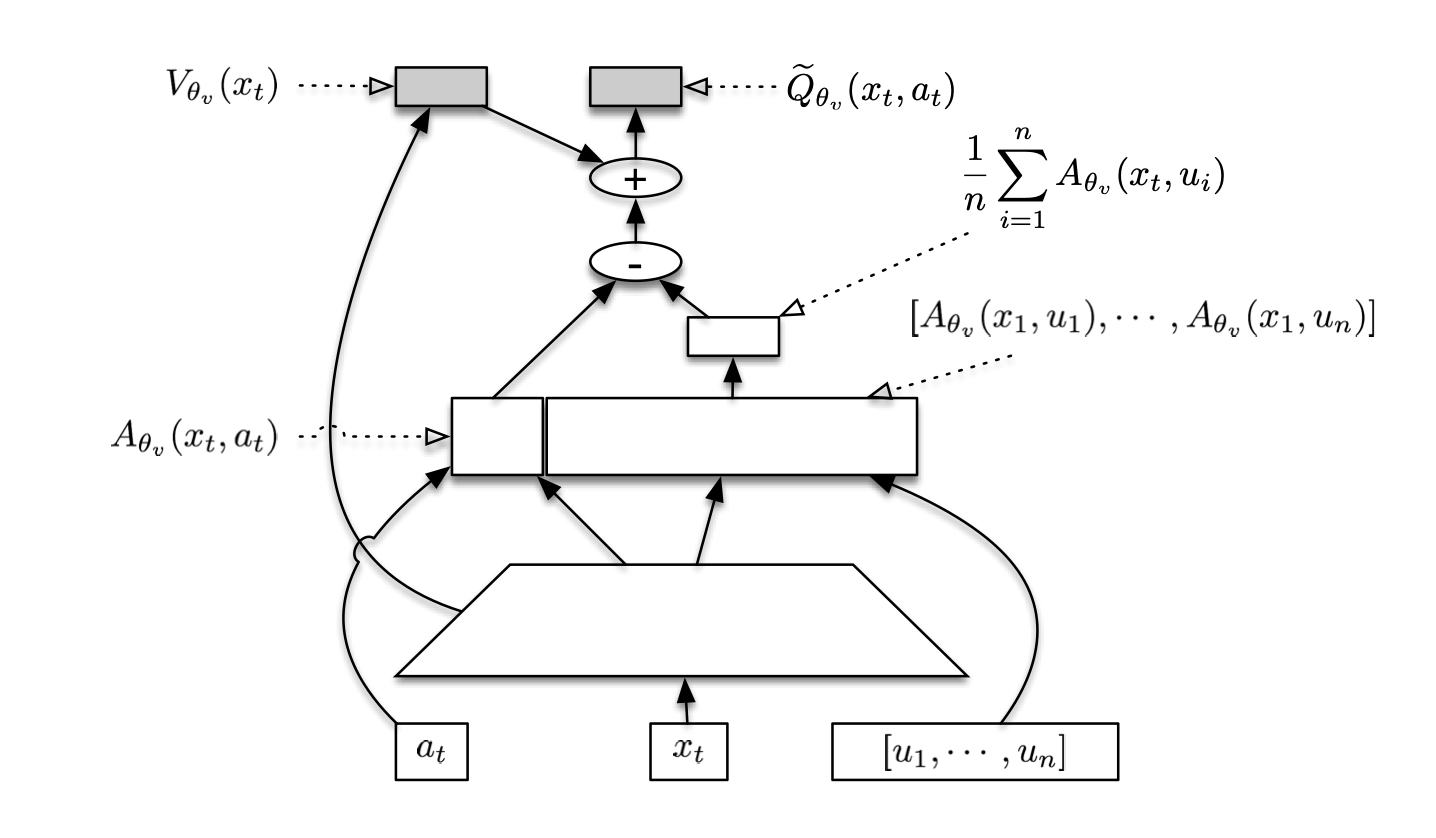
\includegraphics[scale=0.5, width=\textwidth]{SDN.png}
\end{figure}

For the continuous case, since it is unpractical to compute value by summing up the action-values, 
we should deterministically get output from the critic network.
To acheive this, the paper uses a Stochastic Dueling Network(SDN) to estimate both $V^\pi$ and $Q^\pi$
while maintaining consistency between two estimates.(see Figure 1)

The corresponding estimate for $Q^\pi$ of SDN is computed as follows:
\[
  \tilde{Q}_{\theta_v}(x_t, a_t) \sim V_{\theta_v}(x_t) + A_{\theta_v}(x_t, a_t) - \frac{1}{n}\sum_{i = 1}^n A_{\theta_v}(x_t, u_i), \text{where } u_i \sim \pi(\cdot | x_t)
\]
To train the network, the paper as well uses $Q^{ret}$ for target action-value.
For the state value $V^\pi$, they uses the following target:
\[
    V^{target}(x_t) = \min\{1, \frac{\pi(a_t|x_t)}{\mu(a_t | x_t)}\} (Q^{ret}(x_t, a_t) - Q_{\theta_v}(x_t)) + V_{\theta_v}(x_t)
\]
, which is derived by applying the trunction and bias correction trick like what have been done on the policy gradient update.

For continous trust region updating, the paper replaced $Q^{ret}$ with $Q^{opc}$, 
which is basically $Q^{ret}$ without truncated importance ratio.
Though might resulting in a less stable learning, $Q^{opc}$ could better utilize the returns since its not truncated.
The choice is made since by experiment they found out that $Q^{opc}$ often leads to faster learning on continous cases.
